% ============================================================
%  N.2.3  DepFiN CS4: PE Aspect Ratio Sweep
% ============================================================
\subsection{DepFiN: PE Aspect Ratio (CS4)}
\label{sec:cs4-aspect}

\subsubsection{Motivation}

CS4 fix the total number of PEs at
2\,048 and varying only the aspect ratio, from the extremely
column-heavy configuration $2 \times 1\,024$ to the extremely
row-heavy configuration $1\,024 \times 2$.
Memory sizes and register capacities are held constant at the
per-workload values used throughout the DepFiN experiments.

Because rows map to output channels~$Z$ and columns map to tile
width~$Q$, shifting PEs from columns to rows simultaneously reduces
the tile size and increases the $Z$-parallelism.
The tile size, in turn, is chosen for the experiment as the largest divisor
of~$Q$ that fits within the available columns.
A strongly column-heavy shape therefore wastes rows (few $Z$ channels
processed per pass, many re-reads of input activations from the
Feature Memory), while a strongly row-heavy shape wastes columns (tiny
tile, many DRAM-level passes, many weight re-reads from the Weight
Memory).
The EDP curve is thus expected to be U-shaped, with a minimum at the
aspect ratio that best balances the two effects.

\subsubsection{Results}

Figure~\ref{fig:depfin-cs4} shows EDP (log scale, primary axis) and
energy ($\mu$J, linear scale, secondary axis) as a function of aspect
ratio for each workload.
The gold star marks the EDP-optimal configuration.

\begin{figure}[htbp]
  \centering
  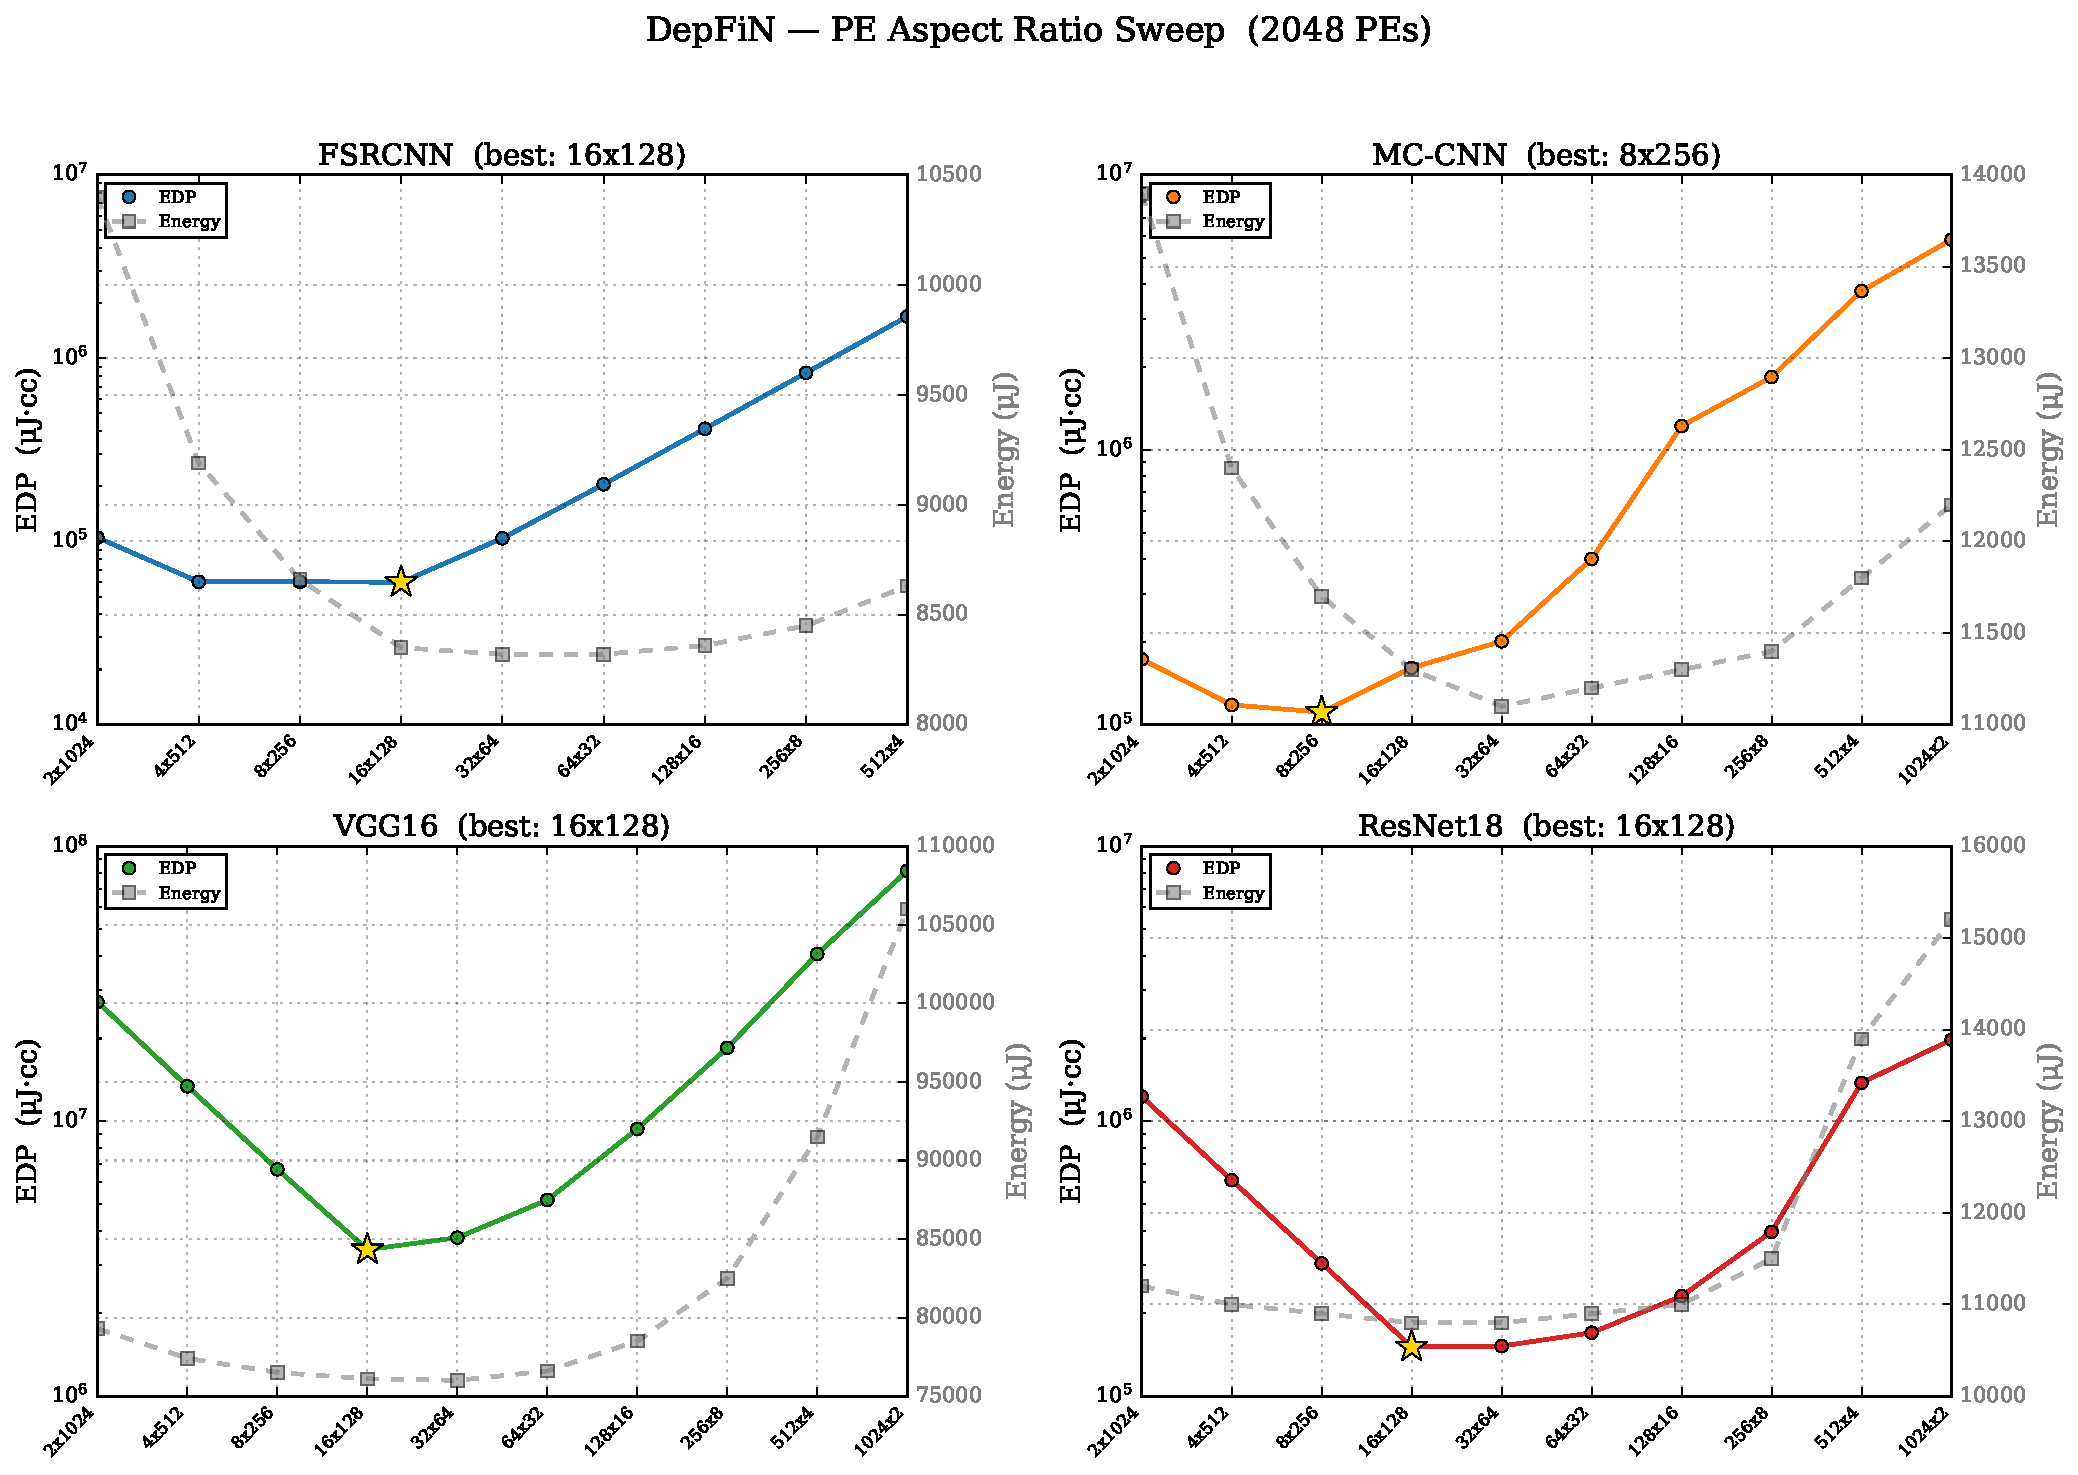
\includegraphics[width=0.9\textwidth]{plots/depfin_cs4_aspect_ratio.pdf}
  \caption{DepFiN CS4: EDP and energy vs.\ PE aspect ratio
    (total PEs\,=\,2\,048).
    The gold star marks the minimum-EDP configuration.}
  \label{fig:depfin-cs4}
\end{figure}

\paragraph{FSRCNN (activation-dominant).}
The EDP curve exhibits a broad minimum centred on $16 \times 128$
($5.59 \times 10^{4}$\,J$\cdot$cc), with the neighbouring
configurations $4 \times 512$ and $8 \times 256$ within
5\,\% and 3\,\% respectively.
Moving toward the row-heavy end the EDP rises steeply: at $512 \times 4$, the increase is driven entirely by latency, which grows by $28\times$
from $16 \times 128$ configuration to $512 \times 4$, as the tile
shrinks from 120 (the maximum with 128 PE Columns) to 4 and each additional DRAM pass reloads the full weight set.
Energy, in contrast, varies by only $\pm 20$\,\% across the entire
sweep, confirming that for activation-dominant workloads the dominant energy
component, register-level operations, is largely insensitive to the
array shape.

\paragraph{MC-CNN (activation-dominant).}
MC-CNN is the only workload whose optimum shifts away from
$16 \times 128$: the best configuration is $8 \times 256$.
The shift occurs because MC-CNN's output spatial dimension
($Q = 1\,242$) benefit from the wider tile that 256
columns provide, reducing DRAM-level passes beyond what 128 columns
can achieve.
At the column-heavy extreme ($2 \times 1\,024$) the EDP is
$1.7\times$ worse, while at the row-heavy
extreme ($1\,024 \times 2$) it is
$53\times$ worse, making the U-shape strongly
asymmetric: the penalty for too many rows far exceeds the penalty for
too many columns.

\paragraph{Weight-dominant workloads (VGG16, ResNet18).}
Both workloads are optimized at $16 \times 128$.
VGG16 EDP drops sharply from $2 \times 1\,024$ to $16 \times 128$ with an $8\times$ improvement, then rises again at $1\,024 \times 2$ configuration, $24\times$ worse than the optimum.

The left-hand descent is driven by latency: at $2 \times 1\,024$ only
two output channels are mapped per pass, requiring many temporal
iterations over~$Z$, while at $16 \times 128$ the bottleneck layer's
channel count (64) is covered in four passes.
The right-hand ascent is driven by both latency and energy: as columns
shrink below 128 the tile fragments, weight memory re-reads multiply, and
energy increases by $+42$\,\%.
ResNet18 mirrors this pattern, with the EDP at the row-heavy extreme
$13\times$ above the optimum.

\paragraph{Considerations.}
All four workloads produce a U-shaped EDP curve, confirming that both
extremes of the aspect ratio are detrimental.
The optimum lies near $16 \times 128$ for three of the four workloads
and at $8 \times 256$ for MC-CNN, whose large output spatial dimension
rewards a wider tile.
The curve is consistently asymmetric: but the rapidity of growing of EDP is determined by the activation or weight dominance of the workload.

